% Template for ApJ-type papers

\documentclass[12pt,preprint]
%{aastex}
{emulateapj}

\usepackage{rotating}
\usepackage{amssymb,amsmath}
%\usepackage{graphicx}[subfloat]
\usepackage{multirow}
\citestyle{aa}

\bibliographystyle{apj_w_etal}

\newcommand{\vect}[1]{\mathbf{#1}}
\newcommand{\xad}{\vect{x}}

\newcommand{\vdag}{(v)^\dagger}
\newcommand{\myemail}{jaguirre@nrao.edu}
\newcommand{\lsim}{{_{<}\atop^{\sim}}}
\newcommand{\gsim}{{_{>}\atop^{\sim}}}
\newcommand{\etal}{{et al.\/}}
\newcommand{\ie}{{\em ie.\/}}
\newcommand{\cmq}{cm{$^{-3}$}}
\newcommand{\per}{$^{\rm{-1}}$}
\newcommand{\tc}{{$\theta^1$~Orionis~C}}
%\newcommand{\msol}{M{$_{\odot}$}}
\def\msol{\ifmmode {\>M_\odot}\else {$M_\odot$}\fi}
\newcommand{\lsol}{L{$_{\odot}$}}
\newcommand{\kms}{km~s{$^{-1}$}}
\newcommand{\hii}{H~{\sc ii}}
\newcommand{\Hii}{H~{\sc ii}}
\newcommand{\Ha}{\mbox{H$\alpha$}}
\newcommand{\sii}{S~{\sc ii}}
\newcommand{\Feii}{Fe~{\sc ii}}
\newcommand{\oi}{O~{\sc i}}
\newcommand{\nii}{N~{\sc ii}}
\newcommand{\oiii}{O~{\sc iii}}
\newcommand{\mgii}{Mg~{\sc ii}}
\newcommand{\tco}{{$^{13}$CO}}
\newcommand{\CO}{{$^{12}$CO}}
\newcommand{\Tco}{{$^{12}$CO}}
\newcommand{\co}{C{$^{18}$O}}
\newcommand{\Lsol}{L$_{\odot}$}
\newcommand{\Msol}{M$_{\odot}$}
%\newcommand{\C18o}{C$^{18}$O($1\rightarrow 0$)}
\newcommand{\Check}{{\bf ???}}
\newcommand{\mum}{\ensuremath{\mu \mathrm{m}}}
\newcommand{\flux}{flux density}
\newcommand{\solar}{\ensuremath{\odot}}

\newcommand{\epsi}{\varepsilon}
\newcommand{\herschel}{{\em Herschel}}


\newcommand{\TBD}{{\bf TBD}}

\def\Figure#1#2#3#4{
\begin{figure}[htb]
\epsscale{#4}
\plotone{#1}
\caption{#2}
\label{#3}
\end{figure}
}

\def\Table#1#2#3#4#5{
\begin{deluxetable}{#1}
\tablewidth{0pt}
\tablecaption{#2}
\tablehead{#3}
\startdata
\label{#4}
#5
\enddata
\end{deluxetable}
}

\newcommand{\cii}{[C{\sc ii}]}
\def\hi{H{\sc i}}
\newcommand{\smg}{SMG}
\newcommand{\smgs}{SMGs}

\newcommand{\penn}{1}
\newcommand{\jpl}{2}
	% End definitions


\shorttitle{Measuring galaxy clustering with Far-IR line intensity mapping}
\shortauthors{Ugzil, Aguirre \& Bradford}

\begin{document}

\title{Measuring galaxy clustering with Far-IR line intensity mapping}

\author{B.~D.~Uzgil\altaffilmark{\penn}}

\author{J.~E.~Aguirre\altaffilmark{\penn}}

\author{C.~M.~Bradford\altaffilmark{\jpl}}

\email{badeu@sas.upenn.edu}

\altaffiltext{\penn}{University of Pennsylvania, Philadelphia, PA 19104}

\altaffiltext{\jpl}{Jet Propulsion Laboratory}

\begin{abstract}

Three dimensional (3D) measurements of galaxy clustering provide rich information about the process of galaxy formation and evolution, linking the theoretical structure of dark matter halos to the masses, types, luminosities, star formation rates, and numbers of galaxies inhabiting them at any epoch.  The largest such surveys to date have been conducted using optically selected galaxies discovered in photometric surveys, followed up by spectroscopy.  At redshifts $z>1$, however, the cosmic star formation rate becomes dominated by extremely dusty systems, and the appropriateness of using optically selected galaxies to study the clustering properties of these dusty star-forming galaxies (DSFGs) is suspect.  Far-infrared lines are excellent unextincted tracers of the physics of the ISM and of star formation, but it is technically daunting to produce redshift surveys using these lines which will attain the necessary density to make precision measurements of the 3D clustering function.  In this paper, we explore a new technique to measure galaxy clustering without individual detections of galaxies.  We develop robust predictions of line specific intensity for a suite of astrophysically interesting lines and make predictions about the detectability of the clustering signal via the 3D power spectrum of a data cube, where the galaxies need not be either spatially or spectrally resolved.  We show that line intensity mapping is an efficient method for imaging spectrometers like SPICA/SAFARI to obtain galaxy clustering measurements down to $k<0.1~h$Mpc$^{-1}$ and out as far as $z\sim3$.
 
\end{abstract}

\keywords{far-infrared spectroscopy; galaxy redshift surveys}

18:11 Pacific 7/20/2013

% - Section 2, in which we discuss the model used for predicting the line power spectra, remains relatively unscathed. Need to keep discussion of lines general, and refrain from using [CII] as a specific example here. Also, will add an intro to the cross power spectrum and the theoretical explanation of the problem of interloper lines at the end of this section.
% 
% - Section 3, the "observational strategy section". Figure 2 will be moved to later in the section. Figures 4, 5, 8 -- the mode counting and SNR vs k plots -- will moved to the beginning. Figure 4 will be changed so that the left-hand point is (0,0) and the k_par and k_perp axes are equal in length. That way, we can identify "k-parallel" or "k-perpindicular" dominated modes as above and below a line drawn at 45 degrees from the origin. We can also plot the region affected by foreground contamination in the k_par-k_perp plane. Figures 6 will be redone to show that with 450 hours, one can measure the [SiII] power spectrum from individually detected sources, but with 45 hours, it is no longer possible to do so, while there is still high S/N on the intensity mapping measurement. We will include a new table that shows the Figure of Merit for the other lines, answering the question "At what z and with which lines is intensity mapping more efficient?"
% 
% - Need to mention that selecting a line is effectively selecting a galaxy type (e.g. high ionization lines for AGN) and so measuring different clustering with the different lines has astrophysical implications. (Are there any references to support why this might be expected to happen, beyond the old "red vs blue" galaxies observation? Thinking off the top of my head, I can imagine it might be possible to detect a different clustering signal for galaxies that are primarily found in merging systems. Not sure how big of an affect this would be in the power spectrum...)
% 
% -Figure 10 needs to make a new point. That is, we must show that the choice of Bethermin model here is robust enough to make valid predictions, based on what is already measured from the cosmic star formation history (Hopkins+Beacom). Also need to show that for lines that have a deficit with respect to LIR and and have a steep LF at the bright end, intensity mapping is useful. (But we have to be careful because [SiII] does not have this deficit with LIR and we have shown intensity mapping to be useful for this line.)

\section{Introduction}

Three dimensional measurements of galaxy clustering provide rich information about the process of galaxy formation and evolution, linking the theoretical structure of dark matter halos to the masses, types, luminosities, star formation rates, and numbers of galaxies inhabiting them at any epoch.  The bulk of such surveys to date have been conducted using optically selected galaxies discovered in photometric surveys, followed up by spectroscopy which identifies lines associated with AGN activity or stellar photospheres (or in some cases with HII regions, e.g., Lyman-$\alpha$ emitters).  At redshifts $z>1$, however, the cosmic star formation rate becomes dominated by extremely dusty systems, and the appropriateness of using optically selected galaxies to study the clustering properties of these dusty star-forming galaxies (DSFGs) is suspect.  

Nevertheless, optical follow-up of DSFGs has yielded some success in obtaining their redshift distribution \citep{chapman05} and clustering \citep{blain}.  The recent watershed of \herschel-detected galaxies has led to intensive study of their properties.  

Intensive optical follow-up, for example of \herschel\ galaxies in \citet{casey12} yielded a relatively small number of galaxies, strongly biased towards low redshift.  Clustering properties of DSFGs have been studied using two-dimensional clustering via a modification of ``$P(D)$'' approach, for example by\citep{bethermin,viero}.  These studies have already shed light on some aspects of the clustering of the most extreme star-forming galaxies $1 < z < 3$, but they are limited by the lack of redshift information, and by the need to include ``nuisance parameters'' in their estimation of the halo model.

From the far-IR to the millimeter, it remains for the future for ALMA or NOEMA to produce redshift surveys with $\sim10^3$ galaxies, or even further down the road for CCAT.  Thus we seek 

% Change focus to measuring the [CII]/FIR relation via knowledge of SFR at z ~ 1

%mention also how the fractions of the CFIRB that are resolved into individual galaxies are low for SPIRE, PACS, and Spitzer maps, so ppl have exploited already statistical methods, P(D) and P(k), with great success. These sources are also going to be the producers of the [CII] emission.

%NOTE: Figure 5 in de Bernardis & Cooray 2012 shows a discrepancy between the Bethermin model and the CLF model, and the authors warn that the redshift parametrization of the L(M_halo) must be reconsidered in future analysis

Atomic (Visbal et al 2011, Gong et al 2012, etc.) and molecular (Lidz et al 2011, etc.) transitions -- such as the 21 cm spin flip transition from H$^{\mathrm{o}}$, CO (2-1), and [CII] 158$\mu$m -- have been investigated as candidates for intensity mapping experiments during the Epoch of Reionization. Of these, the neutral hydrogen case is undoubtedly the most developed in terms of its standing in the literature (cf. Furlanetto, Oh, and Briggs for a review) and in the experimental arena (e.g., PAPER (Parsons et al 2010), MWA), and so interest in measuring the [CII] power spectrum, for instance, has primarily erupted as a means to complement the 21 cm studies at high redshift via the cross-correlation.%\begin{itemize}

A benefit of intensity mapping over individually resolving objects is that the power spectrum is sensitive to the low luminosity galaxies that are below the detection threshold of current and future instruments. Looking forward to EoR, intensity mapping might be the only means available to observe the large population of faint galaxies responsible for reionizing the IGM, given that a telescope such as JWST will only be able to resolve down to 50 percent of UV LF at z ~ 6 (Salvaterra et al 2011). To consider an example at lower redshifts that is \emph{not} intensity mapping but \emph{does} illustrate the potential of power spectra to constrain astrophysically interesting quantities, the SPIRE instrument, even, aboard Herschel misses roughly half of the sources that comprise the cosmic infrared background (CIB) at $z = X.X$ \citep{bethermin12}. In this case, authors exploited a statistical analysis via measuring the clustering term in the angular power spectrum to uncover information about the sources that, 
though unresolved, nevertheless contribute to the intensity fluctuations in the SPIRE 250, 350, and 500 $\mu$m wavebands (Amblard et al 2011). From their analysis, which included a halo model approach to describing the clustering power, they were able to estimate such values relevant to galaxy evolution as characteristic mass for most efficient star formation in a host dark matter halo. With a larger survey area and an added framework to tie galaxy luminosity to the halo model, the clustering amplitude of the CIB power as measured by Herschel was used in conjunction with observed number counts above 0.1 mJy to fit various parameters (Viero et al 2012), including again the halo mass which is most efficient for hosting star formation. Despite the novelty of their approach to interpret the CIB power spectrum, Viero et al 2012 encountered significant difficulty in constraining the parameters of their model with existing data. Indeed, Penin et al (2011) explored the ability of the clustering information from CIB 
angular power spectra to constrain halo model parameters, and found that, while constraints are somewhat improved, simultaneously fitting for clustering data and number counts do not break the degeneracies among the halo model parameters. The authors there and in Viero et al cite unknown redshift distributions of the sources comprising the CIB as the main source of uncertainty in their analyses.

Intensity mapping, on the other hand, contains inherent redshift information encoded along the spectral dimension of the survey volume, and is thus poised to be a valuable complement to current studies of the clustering---and its evolution---of dusty star-forming galaxies at moderate redshift.

Here we examine the value of measuring power spectra of fine structure IR emission lines, including [CII]158\mum,  [NII]\mum, [OI]63\mum, [OIII]88\mum, and [SiII]35\mum, at low to moderate redshifts, specifically between $z = 0.5$ and $z = 3$. As a precursor to Reionization-era experiments, the appeal as a proof-of-principle is obvious, but we focus in this paper on the ability of FIR line intensity mapped power spectra to measure the clustering amplitude of star-forming galaxies. The organization of this paper is as follows. We have calculated the mean emissivity for a suite of IR emission lines based on the IR luminosity function (Bethermin et al 2011) and empirical line to IR luminosity correlations described by Spinoglio et al (2012), and present these results in the context of a power spectrum model in Section 2. In Section 3, we envision suitable platforms---namely the SAFARI instrument aboard future space mission SPICA for the short wavelength lines and a balloon-based experiment for [CII]---for 
conducting the IR intensity mapping and discuss the feasibility of measuring the power spectra with error bar estimates. We also compare intensity mapping to the approach of individual line detections in order to assess its value 
of probing an otherwise undetected population of galaxies. Finally, in Section 4, we present preliminary results on the ability of IR line intensity mapped power spectra to discriminate between halo models. 


%At $z \gtrsim 5$, the UV luminosity function implies that the sources responsible for reionizing the Universe are likely to be very low luminosity ( $ < -16$ AB magnitude) galaxies (Bouwens et al 2011), and intensity mapping has been pointed out as an alternative means of probing these sources which are too faint to be individually detected. The IR luminosity function at moderate redshift depicts the opposite scenario, in which the majority of the IR luminosity is produced by high luminosity sources. 


%Detections of [CII] and other fine structure lines in individual galaxies, such as those from ISO and current observations from Herschel-PACS, provide a view into the ISM of the sources, although confusion limits on PACS restrict observations at $z \gtrsim 1$ to only the brightest galaxies ($L > 10^{XX} L_{\odot}$). The intensity mapping method, in contrast, would not only be sensitive to the fainter population of galaxies, but would also provide a much faster means of observing a large area at a number of redshifts, without distinguishing between individual sources that comprise the intensity fluctuations in the measured power spectrum. We aim to demonstrate in this paper that \emph{the statistical nature of intensity mapping does not limit its ability to probe the ISM of sources} in the surveyed volume. To this end, we derive the average $L_{[CII]}$-$L_{FIR}$ relation for these low-z sources where star formation information is readily available from FUV and IR observations.

%The organization of this paper is as follows. We have calculated [CII], [OI], [NII], and [OIII] power spectra based on the IR luminosity function (Bethermin et al 2011) and empirical line to IR correlations described by Spinoglio et al (2012) during  $0.5 < z <  2$, and present these results in Section 1. In Section 2, we envision suitable platforms for conducting the [CII] intensity mapping experiment and we discuss the feasibility of measuring the power spectra of the lower wavelength lines with SAFARI aboard future space mission SPICA. In Section 3, we perform a maximum likelihood analysis to determine which parameters (e.g. U, hydrogen density, and metallicity) affecting the ISM can precisely determine the line to continuum ratio. 

%, as well as from the conditional luminosity function (CLF, de Bernardis \& Cooray 2012) model of the cosmic far infrared background at the same redshifts and, in Section 1, present predictions for the mean intensity of [CII] across this redshift interval. Using the ancillary star formation rate information, we show (in Section 2) the predicted evolution in the [CII]-FIR relation up to $z = 3$. In order to explore the ability of the power spectrum to probe this relation, we test different assumptions regarding the [CII] production in our theoretical IR sources. Cross-correlation of [CII] with other fine structure lines at the same and nearby redshifts is an interesting means of gaining further insight into the ISM of the detected galaxies and decontaminating the [CII] signal, respectively, which we examine in Section 3. Finally, in Section 4, we envision suitable platforms for conducting the low-redshift [CII] intensity mapping experiment.

%n Section 1, demonstrate the feasibility of characterizing the clustering of dusty, star-formation-dominated galaxies (in comparison to optically selected sources) with this signal. Using the [CII]-FIR and FIR-SFR relations, we also present (Section 2) predictions for a [CII]-generated Madau plot. Such a plot has the unique ability to provide a complete picture of star formation history because the intensity mapping technique is necessarily sensitive to the relatively fainter population of normal galaxies -- in stark contrast to high signal-to-noise detections of spectral lines from traditional observations of single galaxies -- and LIRGs that comprise the majority of the star-forming population up to $z = 1$ (Le Foc'h et al 2004). Finally, in .

 %The intensity mapping method, with its unique sensitivity to the low luminosity population, would provide a means of observing the Universe's SFR transition from a scenario where it is dominated by the normal, low $L_{IR}$ population and the luminous infrared galaxies (LIRGs) to one where roughly 70\% of the cosmic SFR already occurs in ULIRGs in at $z = 1$. This window of time provides a dramatic view into the evolution of the interstellar medium of these galaxies. 


%While there are caveats to the reliability of [CII] as a tracer of FIR luminosity that will be addressed in this letter, the assumption that the galactic FIR luminosity is primarily reprocessed starlight and thus traces star-formation rate (Kennicutt 1998) is sound, given the tight correlation to its well-established optical counterpart, H{$\alpha$} luminosity (Kewley et al 2002, ??? 2012). Furthermore, measuring SFR with a FIR emission line offers the advantage of being unaffected by extinction during a redshift interval where over half of the star formation rate is powered by dusty galaxies with UV extinction  $E(B-V) > 0.25$ magnitudes, as Ly et al (2011) found for galaxies in the Subaru Deep Field., 


%When this result is coupled with the fact that ultraluminous infrared galaxies (ULIRGS, $L_{IR} > 10^{12} L_{\odot}$) contribute roughly 70\% of the star formation rate at $z = 1$ (Le Floc'h et al (2004)

%Have to show how sensitive the pspec is to luminosity

%Ly et al (2011) found that, for the redshift interval $1 < z < 3$, over half (65\%)  formation rate is powered by dusty galaxies with UV extinction $E(B-V) > 0.25$. Indeed, when this result is viewed in the context that the fraction of galaxies contributing to the star formation rate is roughly 70\% ULIRGs


\section{Setting up predictions for Far-IR line power spectra during $0.5 < z < 3$}

Traditional methods for measuring the spatial autocorrelation of galaxies through galaxy surveys rely on the knowledge of the redshift distribution of sources in the survey. Furthermore, they estimate the true three dimensional clustering of galaxies via the angular projection. Intensity mapping, however, contains intrinsic redshift information and provides a direct measure of the clustering power spectrum in three-dimensional k-space, which makes it a highly complementary probe of structure in the cosmic web. 

The complete auto power spectrum of a given FIR line as a function of wavenumber $k$, $P_{i,i}(k,z)$, can be separated into power from the clustering of galaxies, $P_{i,i}^{clust}(k,z)$ and a Poisson term describing their discrete nature, $P_{i,i}^{shot}(k, z)$. We compute the full nonlinear matter power spectrum, $P_{nl}(k, z)$, using the publicly available code HALOFIT+, which has been the standard tool for predicting matter power spectra upon its success in fitting state-of-the-art dark matter simulations over a decade ago (Smith et al 2003) . (We note in passing, however, that since that time, authors (cf., e.g., Takahashi et al 2012) have pointed out improvements to the halo model fit on the small scales previously inaccessible due to constraints on simulation resolution.) The clustering component of the line power spectrum is then written as

%On large scales ($k \lesssim 0.1$ h Mpc$^{-1}$), where the application of linear theory is valid, the clustering power is simply related to the linear matter power spectrum via the halo bias. 
%But, in order to also encompass the clustering on smaller scales that may be relevant in various observational concepts, we calculate the nonlinear matter power spectrum, $P_{nl}(k, z)$, using the publicly available code HALOFIT+, which allows us to write the clustering component as

\begin{equation}
 P_{i,i}^{clust}(k, z) = \bar{S}_{i}^2(z) \bar{b_i}^2(z) P_{nl}(k, z).
 \end{equation}

Here we have implicitly assumed that the fluctuations in line emission trace the matter power spectrum with some average bias, $\bar{b_i}(z)$. The mean line intensity, $\bar{S}_{i}(z)$, in units of Jy sr$^{-1}$, can be calculated as

\begin{equation}
\bar{S}_{i}(z) = \int{\mathrm{d}n_{i} \frac{L_{i}}{4\pi D_L^2}} y_i D_A^2 ,
\end{equation}

where the integration is taken with respect to $n_{i}$, the number of galactic line emitters per cosmological comoving volume element. (The factor $y_i$ is the derivative of the comoving radial distance with respect to the observed frequency, i.e. $y = d\chi/d\nu = \lambda_{i,rest} (1+z)^2/H(z)$, and $D_A$ is the comoving angular distance.)

Finally, the shot noise component of the total line power spectrum---with the same units as the clustering term, namely, Jy sr$^{-1}$(Mpc h$^{-1})^{3}$---takes the form 

\begin{equation} \label{eq:pshot}
P_{i,i}^{shot}(k) = \int{\mathrm{d}n_{i} \left( \frac{L_{i}}{4\pi D_L^2} \right)^2 \left( y_i D_A^2 \right)^2}.
\end{equation}

%employ a halo model (e.g., Cooray \& Sheth, 2002) to write the full clustering component as broken down into contributions from the  the 1-halo and 2-halo terms,

%\begin{equation}
%\begin{split}
%P_{clustering}^{\mathrm{[CII],[CII]}}(k)& = P_{1h} + P_{2h} , \mathrm{where}\\
%P_{1h}& = ...\\
%P_{2h}& = ... ,\\
%\end{split}
%\end{equation}

%which describe the correlations between dark matter in an individual halo and between dark matter in distinct halos, respectively. 

%Generally, given that the infinitesimal cosmological comoving volume element is written $\mathrm{d}V = \mathrm{d}\chi D_A^2 \mathrm{d}\Omega$, where $\mathrm{d}\chi$ is an infinitesimal length along the radial direction, $D_A^2$ is the infinitesimal angular diameter distance, and $\mathrm{d}\Omega$ is the infinitesimal solid angle:

% \frac{\mathrm{d}\chi}{\mathrm{d}\nu
%In the present section, where we utilize [CII] source counts (i.e., $dn_{[CII]}/dS$) from XXX to predict  $n_{[CII}$, the shot noise component of the total [CII] power spectrum takes the form

%\begin{equation}
%P_{shot}^{\mathrm{[CII],[CII]}}(k) = \int{dS \frac{dn_{[CII]}}{dS} \left( \frac{d\chi}{d\nu} D_A^2 \frac{L_{\mathrm{[CII]}}}{4\pi D_L^2} \right)^2}
%P_{shot}^{\mathrm{[CII],[CII]}}(k) = \int{dM \frac{dn_{[CII]}}{dM} \left( \frac{d\chi}{d\nu} D_A^2 \frac{L_{\mathrm{[CII]}}}{4\pi D_L^2} \right)^2}.
%\end{equation} 

%The total [CII] intensity in some volume $V$ at a given redshift is calculated as the number density of [CII] emission from galaxies, $n_{[CII]}$ integrated over the cosmological co-moving volume, $dV = d\chi d_A^2 d\Omega$, where $d\chi$ is an infinitesimal length along the radial direction, $d_A$ is the infinitesimal angular diameter distance, and $d\Omega$ is the infinitesimal solid angle:

%\begin{equation}\label{}
%S^{\mathrm{[CII]}} = \int{\mathrm{d}V \frac{n_{[CII]} L_{\mathrm{[CII]}}}{4\pi D_L^2}} .
%\end{equation}

%Mean specific intensity per steradian is then

%\begin{equation}
%\bar{S}_{\nu, \mathrm{[CII]}} = \int{\frac{\mathrm{d}\chi}{\mathrm{d}\nu} D_A^2 n_{[CII]} \frac{L_{\mathrm{[CII]}}}{4\pi D_L^2} \frac{\mathrm{d}\Omega}{\mathrm{d}\Omega} \frac{\mathrm{d}\nu}{\mathrm{d}\nu}} .
%\end{equation}

\subsection{Calculating IR line volume emissivity}

The number density of line emitters and the line luminosity that appear in equations (2) and (3) can be derived by a variety of methods. In earlier papers on intensity mapping of molecular and fine-structure emission lines at high redshift (z $\gtrsim$ 6), one approach involved using the dark matter halo mass function in lieu of the line emitter density (and invoking a one-to-one correlation between halos and galaxies, which is not unreasonable at high redshifts). The line luminosity, in turn, could be scaled according to the star formation rate, which was related to halo mass via a proportionality constant comprised of factors that described the fraction of baryons available for star formation, as well as the dynamical timescale for star formation. While this theoretical model is feasible at high redshift to provide an estimate on the mean intensity $\bar{S}_i$, we take advantage of the relative wealth of observations of [CII] luminosities in individual galaxies, IR galaxy number counts, and cosmic star formation rate density at the lower redshifts (relevant to this study). To this end, we first employ the empirically-constrained, backwards-evolution model of the IR luminosity function $\Phi(L_{IR}, z)$ from Bethermin et al (2011, hereafter B11) to predict the number of galaxies with luminosity $L_{IR}$ at a given redshift in some comoving volume of the Universe per logarithmic luminosity interval, i.e., $\frac{\mathrm{d}N(L_{IR},z)}{\mathrm{d}V\mathrm{dlog_{10}}L_{IR}}$ or $\frac{\mathrm{d}n_{IR}}{\mathrm{dlog_{10}}L_{IR}}$.  To convert the infrared luminosity to a line luminosity, we apply the relation for $L_{i}$ as a function of $L_{IR}$ provided by Spinoglio et al (2012). The fit in their paper was based on the collection of ISO-LWS observations of local galaxies in Brauher et al (2008), and is reproduced below for the set of lines to be considered in this study: 

\begin{equation}
\begin{split}
L_{\mathrm{[CII]158}}(L_{\mathrm{IR}}) = (0.89 \pm 0.03) \mathrm{log_{10}}L_{\mathrm{IR}} - (2.44 \pm 0.07) \\
L_{\mathrm{[OI]63}}(L_{\mathrm{IR}}) = (0.98 \pm 0.03) \mathrm{log_{10}}L_{\mathrm{IR}} - (2.70 \pm 0.10)  \\
L_{\mathrm{[SiII]35}}(L_{\mathrm{IR}}) = (1.04 \pm 0.05) \mathrm{log_{10}}L_{\mathrm{IR}} - (3.15 \pm 0.16) \\
L_{\mathrm{[OIII]88}}(L_{\mathrm{IR}}) = (0.98 \pm 0.10) \mathrm{log_{10}}L_{\mathrm{IR}} - (2.86 \pm 0.30) \\
\end{split}
\end{equation}

Thus, it becomes possible to write the cosmic mean intensity and shot noise of the line, in units of Jy sr$^{-1}$,  as a function of redshift based on the B11 luminosity function and Spinoglio et al (2012) $L_{i}-L_{\mathrm{IR}}$ relation as

\begin{equation} \label{eq:intensity}
\bar{S}_{\mathrm{i}}(z) = \int_{L_{IR,min}}^{L_{IR,max}} \mathrm{d}L_{IR}  \Phi(L_{IR}, z) \frac{f_{i}}{4 \pi D_{L}^2} \frac{1}{\mathrm{ln}10} y D_A^2
\end{equation}

\begin{equation} \label{eq:pshotlum}
P_{i, shot}(z) = \int_{L_{IR,min}}^{L_{IR,max}} \mathrm{d}L_{IR}  \Phi(L_{IR}, z) \frac{f_{\mathrm{i}}}{4 \pi D_{L}^2} \frac{L_{IR}f_{\mathrm{i}}}{4\pi D_{L}^2} \frac{1}{\mathrm{ln}10} \left(y D_A^2\right)^2
\end{equation}

where $f_{i}$, i.e. $\frac{L_{i}(L_{IR})}{L_{IR}}$, is the fraction of IR luminosity emitted in line $i$, as computed from equation (3). 

It should be noted that the mean line luminosity $\bar{L}_i$ does, in reality, include a contribution from diffuse gas in the intergalactic medium (IGM), yet Gong et al (2012) estimated that the specific intensity of one of the brightest lines typically observed in galaxies, namely [CII],  coming from the IGM ranges from $\sim 10^{-3}$ Jy sr$^{-1}$ to $\sim$ 1 Jy sr$^{-1}$ for different physical conditions in the ISM at $z = 1$---a negligible amount compared to the emission from the interstellar medium (ISM) of galaxies. 

The resulting mean intensities for a variety of FIR lines are plotted in Figure 1 as functions of redshift and observed frequency. $\bar{S}_{\nu}$ vs $\lambda_{obs}$ can be interpreted as identifying the dominant source of fluctuations, according to our model, for a given frequency. As a specific example, if the target line of an observation is [OI]63 at $z = 1$, it will be necessary to distinguish between the target line and contaminants from different redshifts which nonetheless contribute power at the observed frequency. Visbal and Loeb (2010) showed how the cross spectra can be used to differentiate between a target line and a contaminating line (or "bad line", in their words), since emitters at different redshifts will be spatially uncorrelated. The cross power spectrum of two distinct lines can generally be written

\begin{equation}
P_{i,j}(k,z)& = \bar{S}_i(z) \bar{S}_j(z) \bar{b}_i(z) \bar{b}_j(z) P_{nl}(k,z) + P_{shot}^{i,j}(k) %\\
\end{equation}

In the case of far-IR lines, where there is no observational evidence of emitting populations with distinct clustering properties, it is justified to take $\bar{b}_i(z) = \bar{b}_j(z)$. Note that this equality may not hold between the far-IR lines and certain near- and mid-IR lines, which are primarily produced in AGN, and which may have different clustering characteristics.

%Incorporating the IR luminosity function in the approach to estimating the [CII] density facilitates the separation of [CII]-emitting galaxies by luminosity class, i.e., ULIRG, LIRG, or normal galaxy, which is useful since there is not a one-to-one mapping of [CII] luminosity to infrared luminosity for individual galaxies. To understand, then, the relation between [CII] emission from a diverse ensemble of galaxies present in the power spectrum to the star formation rate at a given redshift, it is imperative to sort out the mix of galaxy types and corresponding luminosities that contribute to the total emission. We use the recent compilation of Gracia-Carpio et al. (2011) for the measured relation of $L_{[CII]}$ to $L_{FIR}$ in a range of systems. 

%For most normal galaxies (here taken to mean $L_{FIR} < 10^{11} L_{\odot}$) at any redshift, the $L_{[CII]}/L_{FIR}$ ratio is approximately equal to $3 \times 10^{-3}$ (with a $1-\sigma$ scatter of only $\sim$ 0.3 dex). Since $L_{FIR}$ is well known to tightly correlate with SFR (Kennicutt??), for these systems the $L_{[CII]}$ traces the SFR with a known proportionality constant. 

%In the local universe, dense, high ionization environments are typical of the central star-forming regions of ULIRGs ($L > 10^{12} L_{\odot}$) or LIRGS ($L>10^{11} L_{\odot}$). These environments exhibit underluminous [CII] emission because [CII] is strongly sensitive to the intensity of the UV field and saturates at high UV fluxes. For nearby sources with $L>10^{12} L_{\odot}$, $L_{[CII]}/L_{FIR}$ drops by a factor of $\sim$ 5-10, and $L_{[CII]}$ no longer scales with SFR, but such sources are rare at $z<0.01$ and account for only a small fraction of the total SFR density. Hence, at these redshifts, the bulk of the [CII] emission is from "normal"-type galaxies that obey the relatively tight correlation between $L_{[CII]}-L_{FIR}$. 

%By contrast, at $z \sim 1$, the fraction of SFRD contributed by high luminosity sources substantially increases. At $z = 1-2$, however, the Stacey et al (2010) results show that the threshold for a significant deficiency in $L_{[CII]}$ rises to $L \sim 5 \times 10^{12} L_{\odot}$ (Figure ??), so that the majority of the emission again still adheres to a relatively tight correlation, and the fraction contributed by sources with weak [CII] appears to remain negligible at all redshifts. 

%We can characterize the redshift evolution of $\kappa$ from the IR luminosity function. This behavior is plotted in Figure XXX. 

\begin{figure}[h]
 \centering
 \subfloat(a){
 \label{}
 \includegraphics[width=0.4\textwidth]{b11_spinoglio_intensity_jysr_vs_z.pdf}}
 \subfloat(b){
 \label{fig:bethermin_fir_frac}
 \includegraphics[width=0.4\textwidth]{intensity_vs_lambda_vs_Hz.pdf}}
 \centering
\caption{Intensity of fine structure line emission plotted versus redshift (\emph{top}) and observed wavelength (\emph{bottom}) as predicted from Spinoglio line luminosity fits as applied to the Bethermin (2011) luminosity function.}
\end{figure}

%\begin{equation}
%\bar{L}_{\mathrm{[CII]}} = \int_{L_{IR}^{min}}^{L_{IR}^{max}} \! \mathrm{d}(\mathrm{log_{10}} \, L_{IR}) L_{IR} \Phi(L_{IR}, z) f_{[CII]}(L_{IR}).
%\end{equation}

%The fraction $f_{[CII]}(L_{IR})$ is obtained from the fit for [CII] luminosity---based on local ISO-LWS observations (Brauher et al 2008)---as a function of IR luminosity provided by Spinoglio et al (2011, their equation 33, reproduced below):

%\begin{equation}
%\begin{split}
%f_{[CII]}(L_{IR})& =\frac{L_{[CII]}}{L_{IR}}\\
%                           & =\frac{(0.89 \pm 0.03) \mathrm{log_{10}}L_{IR} - (2.44 \pm 0.07)}{L_{IR}}.
%\end{split}
%\end{equation}

%Finally, in terms of the IR luminosity function, the shot noise becomes

%\begin{multline}
%P_{shot}^{\mathrm{[CII],[CII]}}(k) =  \int_{L_{IR}^{min}}^{L_{IR}^{max}} \! \mathrm{d}(\mathrm{log_{10}}L_{IR}) \, \Phi(L_{IR}, z)\\
%\times  f_{[CII]}(L_{IR}) \left( \frac{L_{\mathrm{[CII]}}}{4\pi D_L^2} \right)^2 \left( \frac{\mathrm{d}\chi}{\mathrm{d}\nu} D_A^2 \right)^2
%\end{multline}

%It should be noted that the mean [CII] luminosity $\bar{L}^{[CII]}$ does, in reality, include a contribution from diffuse gas in the intergalactic medium (IGM), yet Gong et al (2012) estimated that the specific intensity coming from the IGM ranges from $\sim 10^{-3}$ Jy sr$^{-1}$ to $\sim$ 1 Jy sr$^{-1}$ at $z = 1$---a negligible amount compared to the emission from the interstellar medium (ISM) of galaxies. 

\section{Observational Strategy}

We present in this section predictions for the power spectrum of a set of bright far-IR emission lines, namely, [CII]158\mum, [OI]63\mum, [NII]122\mum, [OIII]88\mum, and [SiII]35\mum, and assess sensitivity of envisioned and planned experiments to the power spectra in terms of the signal-to-noise ratio (SNR). These lines, listed in descending order of brightness according to our model predictions in Figure 1, are dominant coolants of interstellar gas in galaxies, arising in either HII regions or FUV irradiated photodissociation regions (PDRs), or, in the case of [CII], both ionized and neutral clouds. (cf., e.g., Osterbrock, Tielens and Hollenbach, for a review of the emitting regions). 

For observing [CII] and [NII], we consider (Section 3.1) a balloon experiment with uninterrupted spectral coverage in the wavelength range 240 to 420 $\mu$m, corresponding to a redshift range for these longer wavelength lines of roughly $0.5 < z < 1.5$. We take the fiducial experimental parameters for the telescope mirror, survey area, and total observing time to be 3.0 m, 1 deg$^2$, and 200 hours, respectively, though we explore the effect of varying the parameters on SNR (cf. Table 1). 

The shorter wavelength lines [OI], [OIII], and [SiII] can be used to extend this redshift range up to $z \sim 3$, as their observed wavelengths fall within the spectral coverage of the SAFARI instrument (30-210$\mu$m) (Roelfsma et al ???) aboard future Japanese space mission SPICA (Nakagawa et al ???); SAFARI will be a part of the Focal Plane Instrument Suite at the time of launch, expected to take place in 2022. We examine the feasibility of measuring the power spectra with SAFARI for a number of observing times and survey areas.

\subsection{$\mathrm{[CII]}158\mum$ and $\mathrm{[NII]}122\mum$}

For concreteness in our discussion of the detectability of the [CII] and [NII] power spectra, we sketch the balloon-borne experiment with different mirror aperture diameters, $D_{ap} = 1.0$ and 3.0 m, and survey  areas, $A_{s} = 0.1, 1.0$, and 10.0 deg$^2$. Relevant parameters for the experimental platforms envisioned here are summarized in Table 1. The fiducial survey parameters, as previously noted, consist of $D_{ap} = 3.0$m, $A_{s} = 1.0$ deg$^2$, and an observing time, $t_{obs}^{tot}$, of 200 hours. 

Predictions for the fiducial case---as computed from the method of combining the cosmological matter power spectrum and the IR LF model outlined in Section 2.1---for the  [CII] power spectrum at four redshifts $z = 0.63, 0.88, 1.16$, and $1.48$ in the above redshift range are shown in Figure 4. (Note that we use  $\Delta_{[CII]}^2 = k^3 P_{[CII], [CII]}(k)/(2\pi^2)$ when plotting the power spectrum, where the integral of $\Delta_{[CII]}^2$ over logarithmic k bins is equal to the variance in real space.) At these redshifts, respectively, the average linear bias has been assumed to be $\bar{b} = 2.0, 2.3, 2.6$, and $2.9$, in line with theoretical predictions from (Cooray and Sheth ???). The crossing of the one-halo and two-halo terms in the power spectrum can be detected with signal to noise at all redshifts.  We calculate error bar estimates and the mean SNR for the power spectrum by assuming a spectrally flat noise power spectrum, so that the noise power in each pixel, $P_{N}$, is calculated from

\begin{equation}
P_N = \sigma_N^2 \frac{V_{pix}}{t_{obs}^{pix}},
\end{equation}

where $\sigma_N^2$ is the instrument sensitivity (noise equivalent intensity, or NEI, in units of Jy sr$^{-1}$ Hz$^{-1/2}$, $V_{pix}$ is the volume of a pixel, and $t_{obs}^{pix}$ is the time spent observing on a single pixel. The variance of a measured $k$, $\sigma^2(k)$, is then written as

\begin{equation}
\sigma^2(k) = \frac{\left({P_{[CII],[CII]}(k) + P_N(k)}\right)^{2}}{N_{mode}},
\end{equation}

where $N_{mode}$ is the number of wavemodes that are sampled for a given $k$ bin of some finite width $\Delta$log(k). (We have chosen $\Delta$log(k) = 0.3 for this analysis.)

The k-averaged SNR, in turn, is calculated from the expression 

\begin{equation}
SNR = \sqrt{\sum_{bins} \left(\frac{P_{[CII],[CII]}(k)}{\sigma(k)}\right)^2}
\end{equation}

Note that It is possible to rewrite $P_N$ in terms of the parameters from Table 1, giving 

\begin{equation}
\begin{split}
P_N& = \sigma_N^2 A_{pix} \Delta r_{los}^{pix} / {\frac{t_{obs}^{survey}}{n_{beams}/N_{instr}^{spatial}}} \\
& = \sigma_N^2 A_{pix}\Delta r_{los}^{pix} /  \frac{t_{obs}^{survey} N_{instr}^{spatial}}{A_{survey}/A_{pix}}\\
& = \sigma_N^2 \frac{\Delta r_{los}^{pix} A_{survey}}{t_{obs}^{survey} N_{instr}^{spatial}}
\end{split}
\end{equation}

In this form, it becomes apparent that---with fixed number of spatial pixels, spectral resolution, and total observing time---the only factor driving up the amplitude of noise power is the survey area; the effect of increasing aperture only allows access to higher wavenumbers. This behavior is shown clearly in Figure 5, where the SNR is plotted as a function of $k$ for different survey geometries and both mirror diameters. Also seen in Figure 5, the greater number of wavemodes sampled (entering as $N_{modes}^{-1/2}$ in the expression for $\sigma$) with the larger survey area does not necessarily compensate for the the increase in $P_{N}$. For example, the factor of ten increase in $P_N$ going from $A_{survey}$ = 1 to 10 deg$^2$ is only overcome by the additional modes in the larger survey area for $k < 1$, leading to a higher S/N for these modes. At $k > 1$, the S/N in each mode for the 1 and 10 deg$^2$ fields becomes comparable. 


\begin {table*}[h]
\begin{center}
\caption {Experimental Parameters for Envisioned Balloon Experiment at $z$ = 0.88} \label{tab:title} 
 \begin{tabular}{ l c c c c c c }
 \hline \hline
  $t_{obs}^{survey}$ (hr)&\multicolumn{6}{c}{200}\\
  $I_{[CII]}$ (Jy sr$^{-1}$)&\multicolumn{6}{c}{6.27 $\times$ 10^3}\\
  NEI (Jy sr$^{-1}$ sec$^{1/2}$)&\multicolumn{6}{c}{2.17 $\times$ 10$^7$}\\
  $B_{\nu}$ (GHz)&\multicolumn{6}{c}{945-1,086}\\
   $\delta_{\nu}$ (GHz)&\multicolumn{6}{c}{2.25}\\
   \hline
  $A_{survey}$ (deg$^2$)&\multicolumn{2}{c}{0.1}&\multicolumn{2}{c}{1.0}&\multicolumn{2}{c}{10.0}\\
  $V_{survey}$ (Mpc$^3$ h$^{-3}$)&\multicolumn{2}{c}{2.87 $\times$ 10^4}&\multicolumn{2}{c}{2.87 $\times$ 10^6}&\multicolumn{2}{c}{2.87 $\times$ 10^8}\\
  \hline
  $D_{ap}$ (m) & 1 & 3 & 1 & 3 & 1 & 3 \\
  Beam FWHM (arcmin) & 0.42 & 1.25 & 0.42 & 1.25 & 0.42 & 1.25 \\
  $V_{voxel}$ (Mpc$^3$ h$^{-3}$) &  19.76 & 2.20 & 19.76 & 2.20 & 19.76 & 2.20 \\
  $t_{obs}^{voxel}$ (hr) & 2.0 $\times$ 10^2 & 2.3 $\times$ 10^1 & 2.1 & 2.3 $\times 10^{-1}$& 2.1 $\times 10^{-2}$ & 2.3 $\times 10^{-3}$\\
  $P_N^{voxel}$ (10$^{10}$ Jy$^2$ sr$^{-2}$ Mpc$^3$ h$^{-3}$)  & 1.17 & 1.17 & 117 & 117 & 11, 700 & 11, 700\\
  \hline
\end{tabular}
\end{center}
\end{table}



%\begin{table}
%\begin{center}
%\begin{tabular}{l c c c}
%\hline
 %& \multicolumn{2}{c}{COSMOS}& Bethermin+Spinoglio \\
%\hline \hline
% & 1.96 deg$^2$ & 0.4 deg$^2$ & \\
%\hline
%SFRD (M$_{\bigodot}$/yr Mpc$^{-3}$) & 0.48 & 0.42 & 0.18 \\
%$\rho_{{IR}}$ (L$_{\textrm {IR}}$ Mpc$^{-3}$) & 2.8 $\times 10^9$ & $2.4 \times 10^9$ & 6.3 $\times 10^8$ \\
%$\rho_{{[CII]}}$ (L$_{\textrm{[CII]}}$ Mpc$^{-3}$) & 4.2 $\times 10^6$ & 3.6 $\times 10^6$ & 7.8 $\times 10^5$ \\
%$\bar{S}_{[CII]}$ (Jy sr$^{-1}$) & 12,000 & 11,000 & 2,600\\
%$P_{shot}$ (Jy sr$^{-1}$) & 1.4 $\times 10^9$ & 1.3 $\times 10^9$ & 2.9 $\times 10^{10}$\\
%\hline
%\end{tabular}
%\end{center}
%\end{table}


\begin{figure*}[h]
\centering
\begin{tabular}{cc}
\includegraphics[width=0.4\textwidth]{pcii_z63_halofit_bethermin_spinoglio_ap3m_1sqdeg_uhp_obs.pdf} &
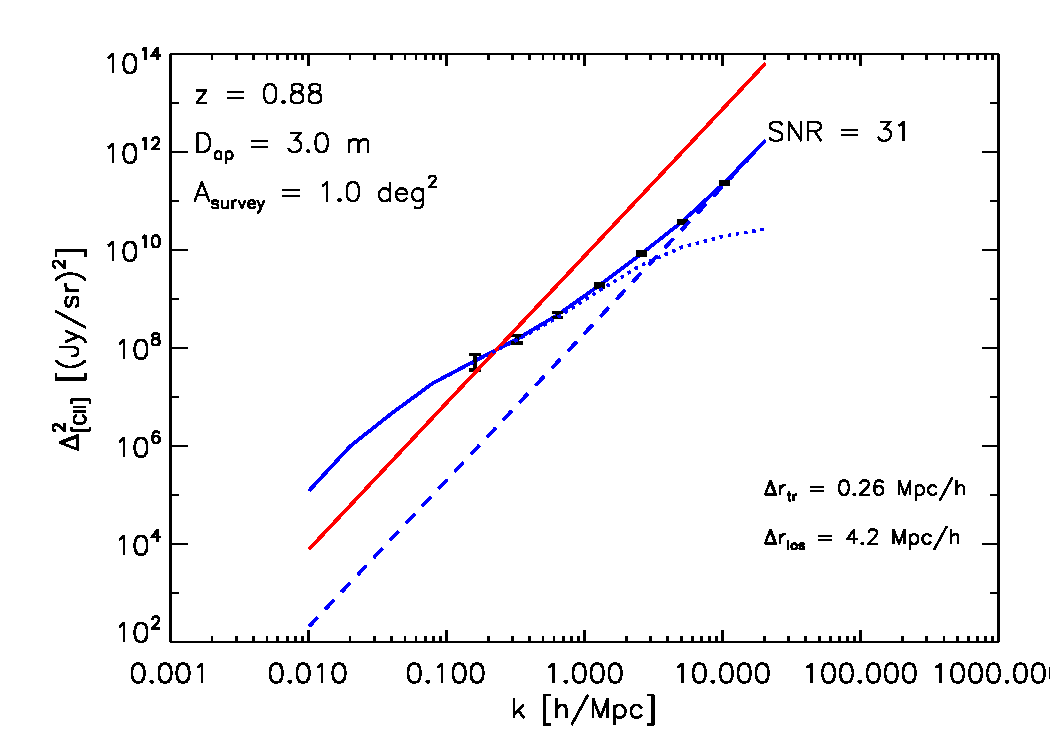
\includegraphics[width=0.4\textwidth]{pcii_z88_halofit_bethermin_spinoglio_witherror_constlogk_ICarISkmodes_ap3m_1sqdeg_uhp_obs.pdf} \\
\includegraphics[width=0.4\textwidth]{pcii_z116_halofit_bethermin_spinoglio_ap3m_1sqdeg_uhp_obs.pdf} &
\includegraphics[width=0.4\textwidth]{pcii_z148_halofit_bethermin_spinoglio_ap3m_1sqdeg_uhp_obs.pdf}
\end{tabular}
\caption{\label{} Predicted [CII] power spectra with error estimates from $z$ = 0.63 to $z$ = 1.48 for telescope with 3 meter aperture and a survey area of 1 square degree. Blue, green, magenta, and cyan curves denotes power spectra computed with upper limits of $L_{IR} = 10^{13}, 10^{12}, 10^{11}$, and 10$^{10}$ L$_{\odot}$, respectively.}
\end{figure}

\begin{figure}[h]
\centering
\begin{tabular}{cc}
\includegraphics[width=0.25\textwidth]{kbin4hist_1sqdeg_z88} &
\includegraphics[width=0.25\textwidth]{kbin5hist_1sqdeg_z88}} \\
\includegraphics[width=0.25\textwidth]{kbin6hist_1sqdeg_z88}} &
\includegraphics[width=0.25\textwidth]{kbin7hist_1sqdeg_z88}} \\
\includegraphics[width=0.25\textwidth]{kbin8hist_1sqdeg_z88}} &
\includegraphics[width=0.25\textwidth]{kbin9hist_1sqdeg_z88}} \\
\includegraphics[width=0.25\textwidth]{kbin10hist_1sqdeg_z88}} \\

\end{tabular}
\caption{\label{} Sample histogram of $k_{par}$-$k_{perp}$ for the fiducial [CII] experiment at $z=0.88$.}
\end{figure}

\begin{figure}[h]
\centering
\begin{tabular}{cc}
\includegraphics[width=0.25\textwidth]{kbin3hist_10sqdeg_z88} &
\includegraphics[width=0.25\textwidth]{kbin4hist_10sqdeg_z88} \\
\includegraphics[width=0.25\textwidth]{kbin5hist_10sqdeg_z88}} &
\includegraphics[width=0.25\textwidth]{kbin6hist_10sqdeg_z88}} \\
\includegraphics[width=0.25\textwidth]{kbin7hist_10sqdeg_z88}} &
\includegraphics[width=0.25\textwidth]{kbin8hist_10sqdeg_z88}} \\
\includegraphics[width=0.25\textwidth]{kbin9hist_10sqdeg_z88}} &
\includegraphics[width=0.25\textwidth]{kbin10hist_10sqdeg_z88}} \\

\end{tabular}
\caption{\label{} Sample histogram of $k_{par}$-$k_{perp}$ for the [CII] experiment at $z=0.88$. Parameters are the same as in the previous figure, with the exception of a larger survey area, $A_{survey}$ = 10.0 deg$^2$.}
\end{figure}

%\begin{figure*}[h]
%\centering
%\begin{tabular}{cc}

%\includegraphics[width=0.5\textwidth]{pcii_z63_halofit_bethermin_spinoglio_witherror_constlogk_ICarISkmodes_ap1m_1sqdeg_uhp_obs.pdf} &
%\includegraphics[width=0.5\textwidth]{pcii_z88_halofit_bethermin_spinoglio_witherror_constlogk_ICarISkmodes_ap1m_1sqdeg_uhp_obs.pdf} &
%\includegraphics[width=0.5\textwidth]{pcii_z116_halofit_bethermin_spinoglio_witherror_constlogk_ICarISkmodes_ap1m_1sqdeg_uhp_obs.pdf} &
%\includegraphics[width=0.5\textwidth]{pcii_z148_halofit_bethermin_spinoglio_witherror_constlogk_ICarISkmodes_ap1m_1sqdeg_uhp_obs.pdf} &
% \end{tabular}
% \caption{Predicted [CII] power spectra  from $z$ = 0.63 to $z$ = 1.48 for telescope with 1 meter aperture and a survey area of 1 square degree.}
%\end{figure}

%We calculate the mean signal to noise ratio (SNR) for each power spectra

%Detectability of the power spectra is assessed by comparing the signal-to-noise ratio (S/N) as a function of wavenumber (Figure 3). 

\begin{figure}[t]
\centering
\begin{tabular}{cc}
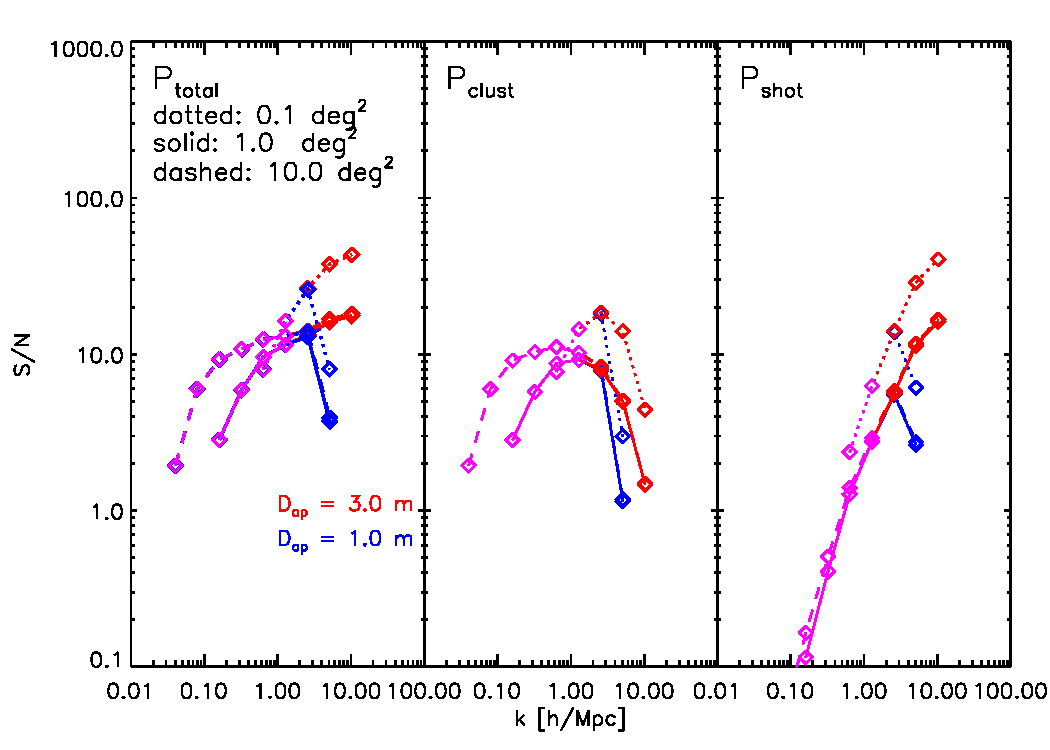
\includegraphics[width=0.4\textwidth]{snr_tot_clust_shot_vs_kbin_apertures_asurveys_z88} \\
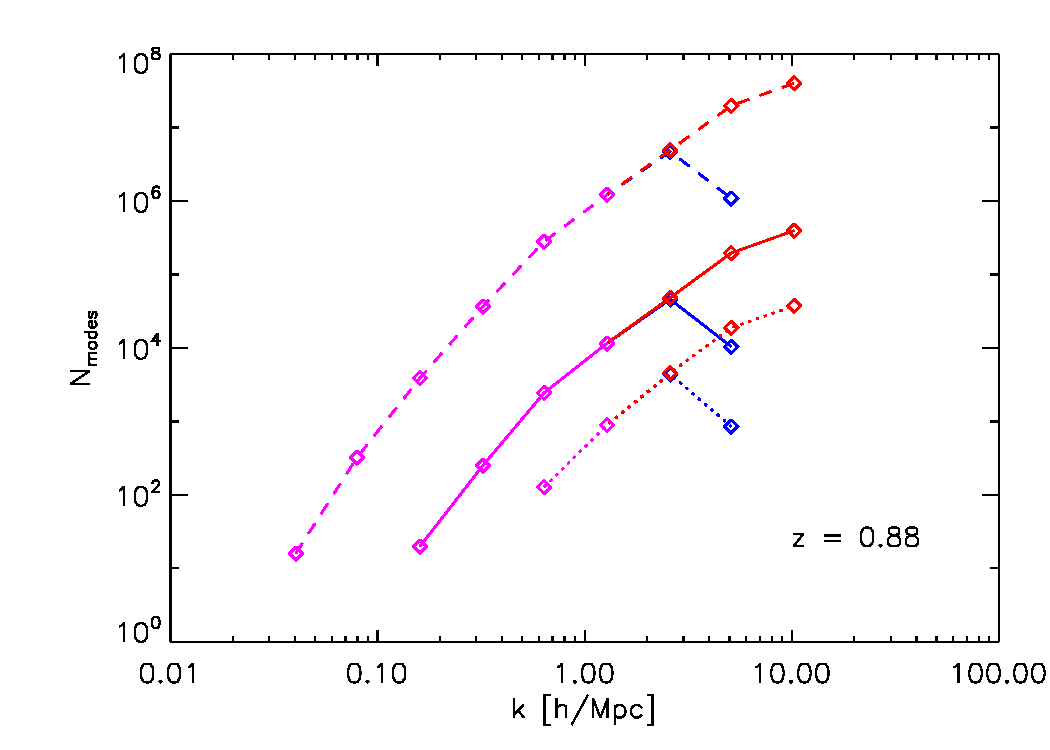
\includegraphics[width=0.4\textwidth]{nmode_vs_kbin_apertures_asurveys_all_z88.pdf} \\
\end{tabular}
\caption{\label{} Signal to noise on the dimensionless [CII] power spectrum $\Delta_{\textrm{[CII]}}^2$ and number of modes as a function of $k$. The blue lines represent S/N for the 1 meter aperture, red denotes a 3 meter aperture, and purple shows where the two overlap. Survey areas of 0.1, 1, 10 square degree fields are shown as the solid, dashed, and dotted lines, respectively. The special case of a line scan survey with dimensions 1 degree by 1 beam for a 3 meter aperture is plotted as the dash-dotted line.}
\end{figure}



\subsection{$\mathrm{[OI]63, [OIII]88}$, and $\mathrm{[SiII]35}$}

The [OI], [OIII], and [SiII] power spectra are shown in Figure 8. For each line, we examine the effect of survey area and observing time on the total, clustering, and shot noise power spectrum. We also explore the effect of changing $L_{IR, min}$ in equations \eqref{eq:intensity} and \eqref{eq:pshotlum}, in an effort to understand when the technique of intensity mapping may be advantageous to constructing a power spectrum from individually detected galaxies. To this end, we compare an $L_{IR,min}^{\mathrm{SAFARI}}$ corresponding to the faintest galaxy detectable (i.e., SNR of the line is $5-\sigma$) with SAFARI to the $L_{IR, min}$ probed by intensity mapping, which, in theory, is simply the natural lower limit in the IR luminosity function, taken to be 10$^8$ L$_{\odot}$. We use two values for $L_{IR,min}^{\mathrm{SAFARI}}$, where the faintest detectable galaxy is calculated from $t_{obs}^{pix} = 1$ and 0.1 hr (Table ???).  

\subsection{Effect of varying $L_{IR, min}$}

The increase in survey area provides higher signal to noise in the lower $k$s needed to probe clustering on galactic scales. A survey area of 2 deg$^2$ corresponds to a fundamental mode of ~ 0.1 h/Mpc. In Figure ???, we calculate the power spectrum for [OI]63, varying the scale of the fundamental mode probed by the hypothetical survey. We go down to scales of 0.03 h/Mpc, but it should be kept in mind that modes smaller than 0.08h/Mpc will likely be lost to continuum foreground cleaning. 

In the case of the bright lines [OI]63 and [OIII]88, under condition that $t_{obs}^{pix} = 1.0$ hr, the effect of replacing $L_{IR,min}$ with $L_{IR,min}^{\mathrm{SAFARI}}$ on the total power spectrum (leftmost panels, Figure 8) is barely noticeable. This is because $L_{IR,min}^{\mathrm{SAFARI}}$ is only a factor 0.958 times smaller than the characteristic luminosity $L^{*}$ for [OI]63 at $z = 1.5$, and a factor 1.45 larger for [OIII]88 at $z = 1.16$, resp. Since the majority of the signal at these scales comes from the shot noise term, which is weighted heavily by the more luminous sources ($P_{shot} \propto L_{IR}^2$), the resulting change on the power spectrum is negligible. The change in the clustering power is larger, amounting to at most a ??? factor discrepancy at $k = ???$, but all modes of the power spectra are detectable with high SNR in both cases.

After cutting $t_{obs}^{pix}$ from 1 hr to  0.1 hr, the detectability of the clustering power spectrum changes appreciably when replacing $L_{IR,min}$ with $L_{IR,min}^{\mathrm{SAFARI}}$, resulting in a maximum of ??? times lower amplitude in the clustering term at $k =$ ??? h/Mpc. This decrease in the amplitude pushes the SNR on the clustering below unity. In comparison, the SNR on the clustering power with $L_{IR, min}$ = 10$^8$ L$_{\odot}$ ranges from $\sim 3$ to as high as $\sim 10$ across all $k$ modes. We note that the additional SNR on the power spectrum with ten times longer integration time per pixel only amounts to less than $1-\sigma$ increase in the significance of detection for the lowest $k$ modes, which probe physical scales corresponding to the intersection of the 1-halo and 2-halo terms. In this brief ``cost-benefit analysis," we are led to conclude that intensity mapping is a more efficient means of measuring the clustering power spectrum, compared to reconstructing the power spectrum from time-consuming galaxy surveys. 

We now turn to the line [SiII]35. This line is fainter in comparison to [OI]63 and [OIII]88 and so would require a great deal more integration time to reach comparable significance in a detection. Given only 1 hr or 0.1 hr per pixel, a comparable significance can only be obtained for the most luminous systems: $L_{IR} = 4 \times 10^{12}$ or $1 \times 10^{13}$ L$_{\odot}$, resp. Thus, the SNR on the clustering power spectrum, which is sensitive to the mean of the luminosity function, is as low as $???$ when integrating down to $L_{IR,min}^{\mathrm{SAFARI}}$. While integrating down to $L_{IR,min}$ does significantly improve the SNR, the signal is intrinsically low enough so that SNR on the clustering power spectrum remains subunity at all scales for all survey size and integration time combinations, except for attaining SNR $\sim 2-4$ for $A_{s} = 2$ deg$^2$ and $t_{obs}^{pix} = 1$ hr (i.e, $t_{obs}^{survey} = 1800$ hr). The SNR on the shot noise power spectrum, however, does fare well even in the case of $t_{obs}^{pix} = 0.1$ hr for all survey sizes only when $L_{IR,min}$; the SNR falls below 1 for $L_{IR,min}^{\mathrm{SAFARI}}$. The change in SNR between $t_{obs}^{pix} = 0.1$ hr and $t_{obs}^{pix} = 1.0 $ hr is also more dramatic for [SiII]. Again, this is understood in terms of the value of $L^{*}$ at that redshift, which is $1.4 \times 10^{12}$ L$_{\odot}$ at $z = 3$. Cutting the $t_{obs}^{pix}$ by a factor of 10 raises the SAFARI detection limit from $L_{IR} = 4.8 \times 10^{12}$ to $1.3 \times 10^{13}$ L$_{\odot}$ \footnote[1]{In the case of [SiII], we adopted $L_{IR, max} = 5 \times 10^{13}$ L$_{\odot}$ in the integral over the IR LF, instead of the value of $10^{13}$ L$_{\odot}$ used for calculations pertaining to other lines.}. This change pushes the threshold much larger than the characteristic luminosity at that redshift, and since sources drop as a Gaussian past $L_{*}$, and since $P_{shot}$ is sensitive to $L_{*}$, the SNR drops as expected for this case. Whereas for the integration down to 10$^8$ L$_{\odot}$ captures more signal and has SNR as high as 70 at $k = 10$ h/Mpc.

\subsection{Effect of varying the fundamental mode}

For [OI]63 at $z = 1.5$, we also study the detectability of the power spectrum in a 450 hr survey of various survey sizes, corresponding to different fundamental modes. Figure $???$ shows the SNR on the total, clustering, and shot noise power spectra (left panel) and the number of modes as functions of $k$. A summary of relevant parameters and results is given in Table $???$.

\begin {table}[h] 
\begin{center}
\caption {Experimental Parameters for SPICA-SAFARI Survey of [OI]63 at $z$ = 1.5} \label{tab:title}
\begin{tabular}{ l c c c c c c  }
\hline \hline
$k_{fund}$ (h Mpc$^{-1}$) & \multicolumn{2}{c}{0.03} & \multicolumn{2}{c}{0.05} & \multicolumn{2}{c}{0.07} \\
\hline
NEI (10$^6$ Jy sr$^{-1}$ sec$^{1/2}$) & \multicolumn{2}{c}{6.2} & \multicolumn{2}{c}{6.2} & \multicolumn{2}{c}{6.2} \\
$A_{survey}$ (deg$^2$) & \multicolumn{2}{c}{44} & \multicolumn{2}{c}{16} & \multicolumn{2}{c}{8.1} \\
 $r_{perp}$ (Mpc h$^{-1}$) & \multicolumn{2}{c}{360} & \multicolumn{2}{c}{220} & \multicolumn{2}{c}{160} \\  
$B_{\nu}$ (GHz) & \multicolumn{2}{c}{360} & \multicolumn{2}{c}{220} & \multicolumn{2}{c}{160} \\
$\Delta \nu$ (GHz) & \multicolumn{2}{c}{4.25} & \multicolumn{2}{c}{4.25} & \multicolumn{2}{c}{4.25} \\
$n_{beams}$ (10$^6$ beams) & \multicolumn{2}{c}{3.3} & \multicolumn{2}{c}{1.1} & \multicolumn{2}{c}{0.61} \\
\hline
$t_{obs}^{survey}$ (hr) & 450 & 1,000 & 450 & 1,000 & 450 & 1,000 \\
\hline
$t_{obs}^{pix}$ (sec) & 40 & 88 & 110 & 240 & 220 & 480 \\
$P_N$ (10$^{10}$ Jy$^2$ sr$^{-2}$ Mpc$^3$ h$^{-3}$) & 12 & 5.3 & 4.2 & 1.9 & 2.2 & 0.97 \\
\hline
\end{tabular}
\end{center}
\end{table}

%\begin{figure}
%\includegraphics[width=0.5\textwidth]{poi63_z1p5_SPICA_bethermin_spinoglio_p5sqdeg_R450_dz0p4_tobs450hr_lirmax.pdf}
%\caption{Predicted [OI]63 power spectra at $z$ = 1.5 for SPICA-SAFARI and survey area $A_{survey}$ = 0.5 deg$^2$ with  $t_{obs}^{survey} = 450$ hr. }
%\end{figure}

\begin{figure}[b]
\centering
\begin{tabular}{cc}
%\includegraphics[width=0.5\textwidth]{pSiII_z3_bethermin_spinoglio_SPICA_p5sqdeg_R450_dz_0p4_tobs450hr_lirmin.pdf} &
%\includegraphics[width=0.5\textwidth]{pSiII_z3_bethermin_spinoglio_SPICA_p5sqdeg_R450_dz_0p4_tobs45hr_lirmin.pdf} 
 \end{tabular}
 \caption{Predicted [SiII]35 power spectra at $z$ = 3 for SPICA-SAFARI and survey area $A_{survey}$ = 0.5 deg$^2$ with  $t_{obs}^{survey} = 450$ hr and 45 hr, resp.}
\end{figure}

\begin{figure}
\centering
\begin{tabular}{}
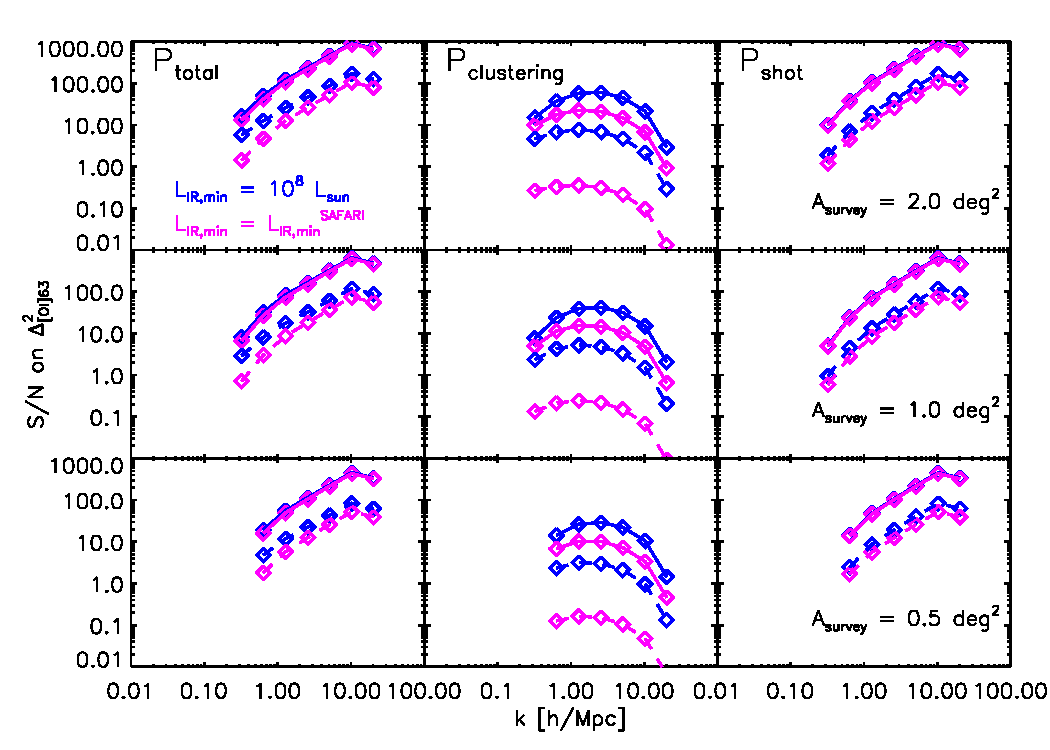
\includegraphics[width=0.5\textwidth]{snr_tot_clust_shot_vs_k_vs_OI63_SPICA_uhp_lirmin_z148.pdf}\\
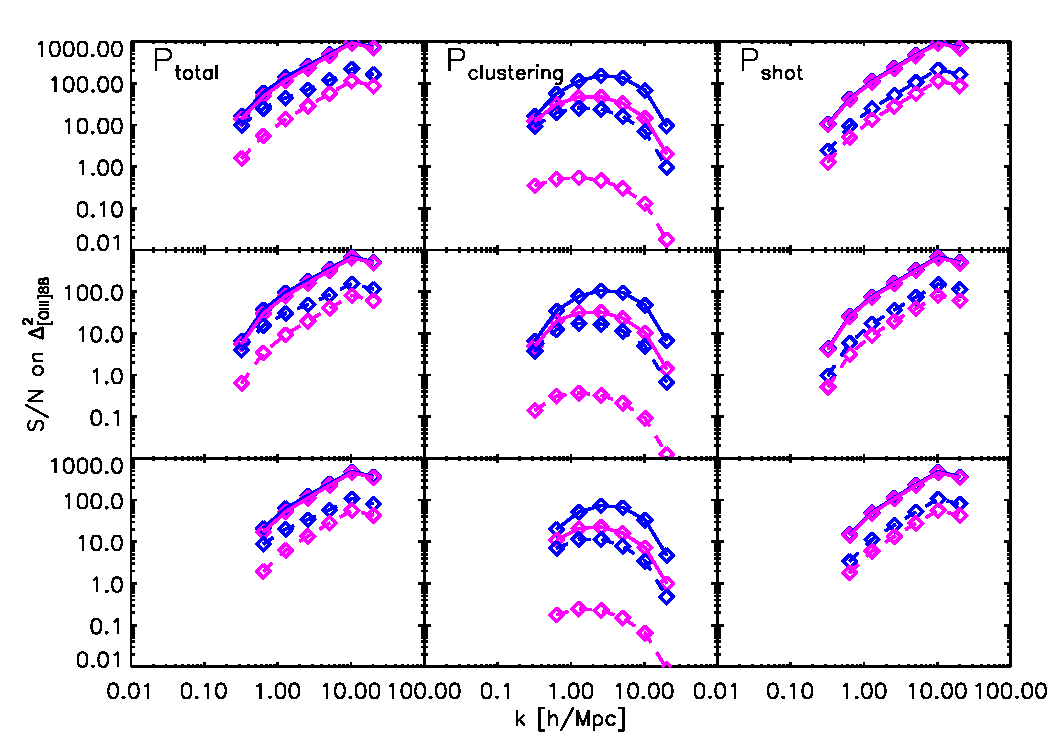
\includegraphics[width=0.5\textwidth]{snr_tot_clust_shot_vs_k_vs_OIII88_SPICA_uhp_lirmin_z148.pdf} \\
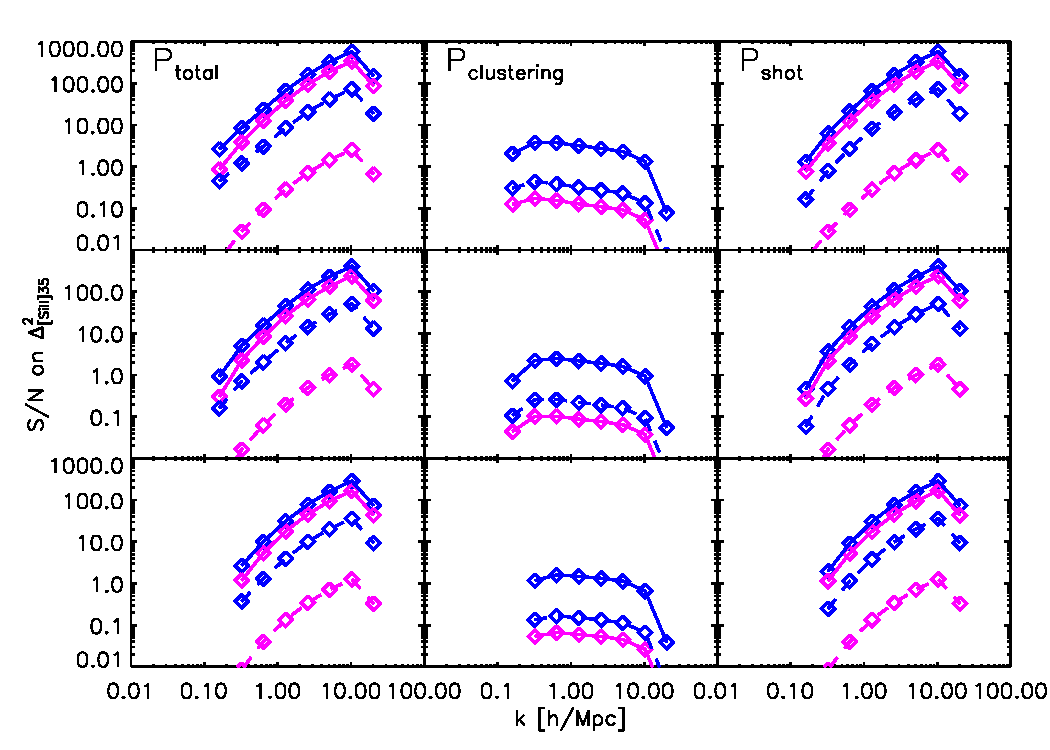
\includegraphics[width=0.5\textwidth]{snr_tot_clust_shot_vs_k_vs_SiII35_SPICA_uhp_lirmin_z148.pdf} \\
\end{tabular}
\caption{\label{} Signal to noise on the dimensionless [OI]63, [SiII]35, and [OIII]88 power spectra $\Delta^2$ for different survey sizes and integration times. Solid curves indicate an integration time per pixel of 1 hour, whereas dashed curves correspond to an integration time per pixel of 0.1 hour.  Blue and magenta curves represent different lower limits in the integration of the IR luminosity function, with blue depicting a lower limit of 10^8 L$_{\odot}$ and magenta depicting the SAFARI detection limit (5$\sigma$). }
\end{figure}

\begin{figure}
\begin{tabular}{cc}
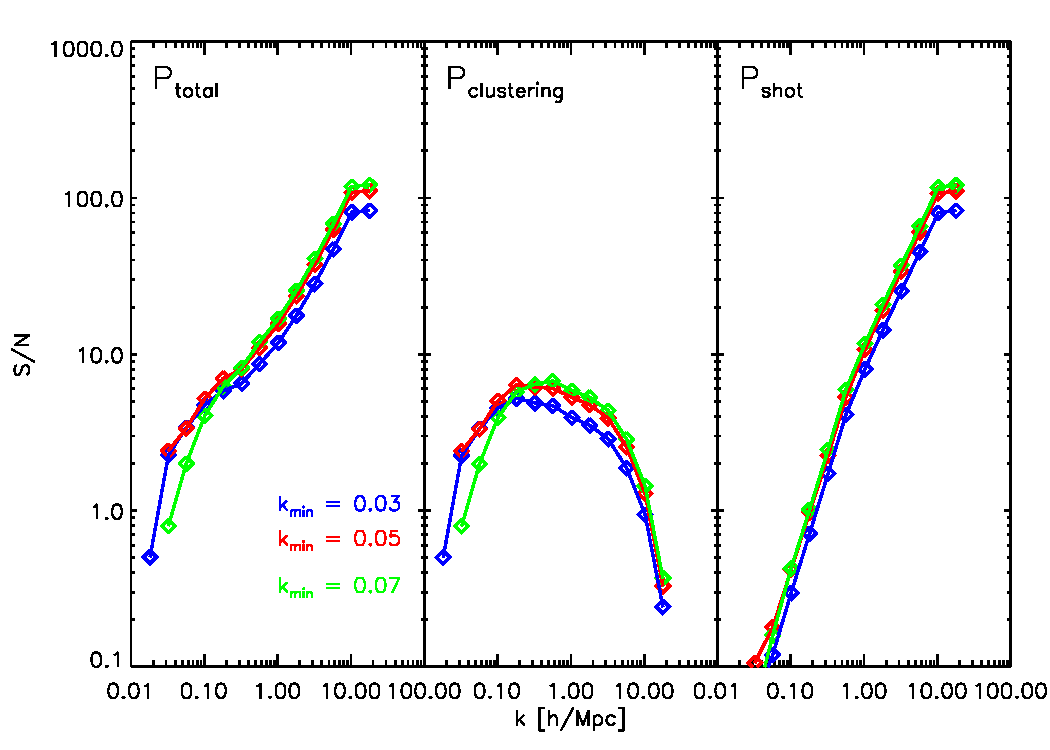
\includegraphics[width=0.4\textwidth]{snr_tot_clust_shot_vs_k_vs_kfund_SPICA_uhp_z148} &
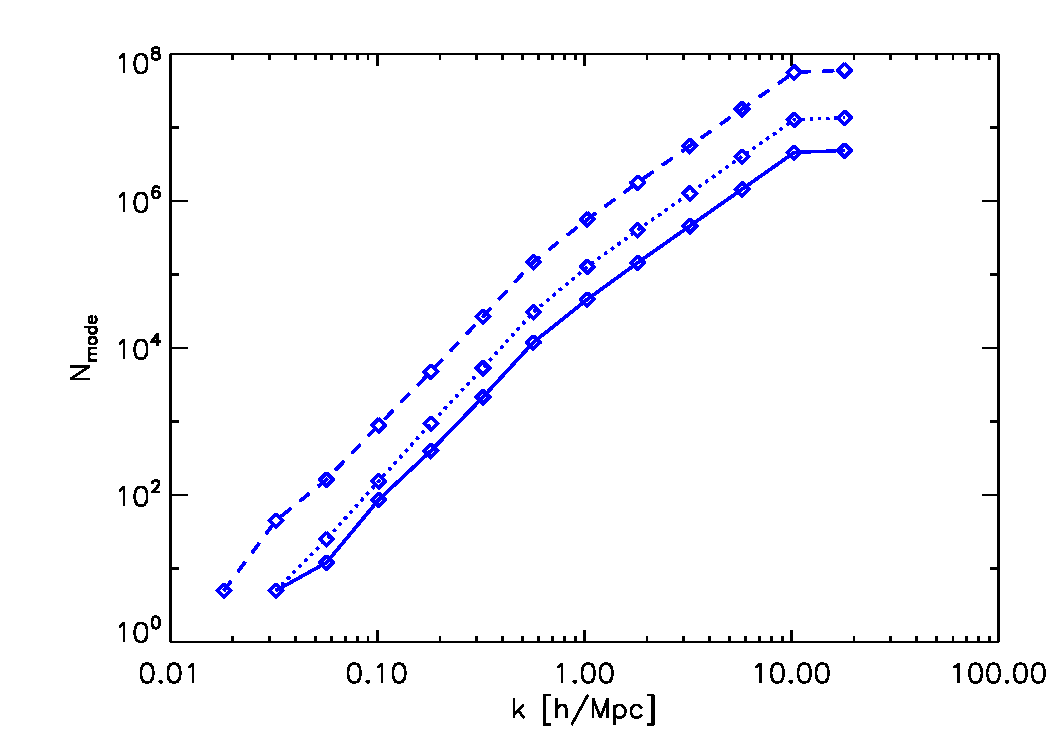
\includegraphics[width=0.4\textwidth]{nmode_vs_k_vs_kfund_SPICA_uhp_z148.pdf}
\end{tabular}
\caption{}
\end{figure}


\subsection{An observer's guide: When to intensity map?}

As a sort of summary, we provide a short discussion on the conditions that most strongly motivate line intensity mapping at the redshifts relevant to this study. There are two basic scenarios when the technique of intensity mapping becomes advantageous to the observer, in lieu of surveys comprised of individually detected galaxies.  

The principal advantage of intensity mapping over individual detections is encapsulated in Figure XXX, which shows predictions of the [SiII]35$\mu$m  power spectrum at $z = 3$ with a mere 45 hours of observing time over a survey area of 0.5 deg$^2$. The power spectrum in this figure is constructed in two ways: (1) with the lower limit of the IR luminosity function fixed at 10$^8$ L$_{\odot}$ (\emph{solid blue curve}) and (2) with the lower limit replaced by the 5$\sigma$-0.1hr detection threshold corresponding to SPICA-SAFARI (\emph{solid magenta curve}). Note that the luminosity function enters into the power spectrum (equation 4) through equations (2) and (5). With 45 hours of observing at $z = 3$, the detection limit for SAFARI is $1.3 \times 10^{13}$ L$_{\odot}$, which means that, according to the Bethermin luminosity function, virtually all [SiII] sources have line luminosities below the threshold for individual detection; at 450 hours of observation (not shown),  the detection limit is $4.4 \times 10^{12}$ L$_{\odot}$ and the percentage of  extragalactic emisson below this threshold is 80\%. (In fact, Spinoglio et al find only a couple of galaxies with normal-type luminosities in their 0.5 deg$^2$ field after 450 hours of integration.) While this missing fraction of the [SiII]-emitting population dramatically diminishes the signal in the power spectrum computed by integrating the luminosity function upwards from the SAFARI sensitivity, the power spectrum computed via intensity mapping, which probes the full range of luminosities in the luminosity function, has relatively high SNR of 40. In this case, intensity mapping becomes an efficient use of telescope observation time, and a unique probe of the low luminosity population. 

\begin{figure}
\begin{tabular}{c}
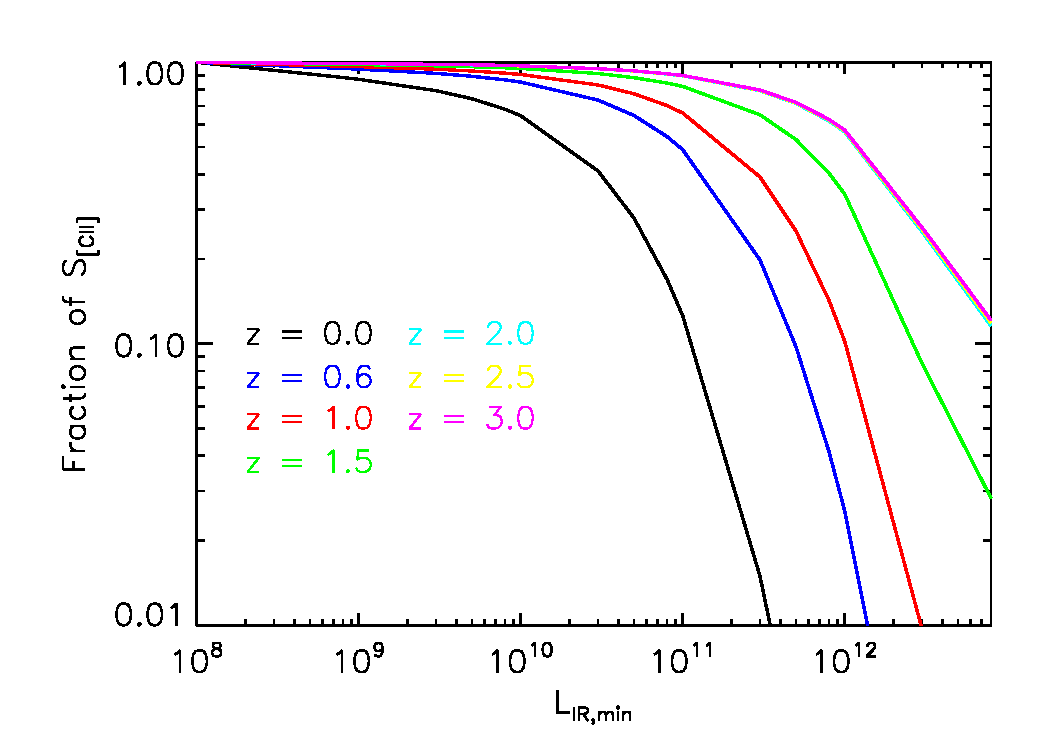
\includegraphics[width=0.4\textwidth]{fraction_cii_emissivity_vs_LIRmin_vs_z.pdf} \\
\includegraphics[width=0.4\textwidth]{fraction_oi63_emissivity_vs_LIRmin_vs_z.pdf} \\
\includegraphics[width=0.4\textwidth]{fraction_SiII35_emissivity_vs_LIRmin_vs_z.pdf} \\
\end{tabular}
\caption{}
\end{figure}

Furthermore, shallow and large area surveys of the FIR emission lines provide a means of connecting large scale structure with galaxy evolution, and intensity mapping can be complementary to individual detections when the area mapped by an observing platform becomes large enough that the required observing time for such a measurement is prohibitive. For example, we consider again the SAFARI instrument aboard SPICA. To map an area of 8.1 deg$^2$, which probes scales down to $k = 0.07$ h/Mpc, with SPICA's 2 arcmin by 2 arcmin field of view would necessitate 7,400 hours of observing time to achieve one hour of integration time per field. If one were to observe the same volume with intensity mapping, on the other hand, it would only be necessary to observe for a relatively modest 450 hours in order to recover high SNR on the power spectrum of a bright line such as [OI]63 (Figure XXX). For comparison, 450 hours of observing via traditional individual detections would amount to 0.06 hr of observing time per field, which means that only galaxies with IR luminosities above $2.3 \times 10^{12}$ L$_{\odot}$ would be observed in [OI]63.

\begin{figure*}
\centering
% \subfloat(a){
% \label{fig:bethermin_sfrd_frac}
% %\includegraphics[width=0.4\textwidth]{bethermin_sfrd_frac.pdf}}
% 
% \subfloat(b){
% \label{fig:bethermin_fir_frac}
% %\includegraphics[width=0.4\textwidth]{bethermin_fir_frac.pdf}}
% 
% \subfloat(c){
% \label{fig:bethermin_cii_frac_rconst}
% %\includegraphics[width=0.4\textwidth]{bethermin_cii_fraction_rconst.pdf}}
% 
% \subfloat(d){
% \label{fig:bethermin_lciilfir_ratio_rconst}
%\includegraphics[width=0.4\textwidth]{bethermin_lciilfir_ratio_rconst.pdf}}
\centering
\caption{\label{fig:multi_panel} Redshift evolution of the star formation rate (a), FIR luminosity (b), [CII] luminosity (c), and $[CII]-L_{FIR}$ relation (d) based on the Bethermin et al (2011) IR luminosity function. In panels (a)-(c), the red, green, and blue colors denote contributions to the luminosity function by ULIRGs, LIRGs, and normal galaxies, respectively, and black lines denote a total. The bottom two panels incorporate two prescriptions for finding $L_{[CII]}$: (1) $L_{[CII]}$ as a function of $L_{IR}$ from Spinoglio et al (2012) (\emph{solid lines}) and (2)  $L_{CII} = 0.003 \times L_{FIR}$ (\emph{dashed lines}). In panel (d), the red, green, and blue line represent the mean $[CII]-L_{FIR}$ for their respective classes. Note there is no externally imposed redshift evolution on the [CII] luminosity in all cases.}
\end{figure*}
% In other words, the red curve depicts $I_{[CII], ULIRG}/L_{FIR, ULIRG},  and similarly for LIRGs (green) and normal (blue) galaxies. The black line represents the average ratio of [CII] to FIR without discriminating the galaxy luminosity class.
%It is thus a worthwhile endeavor to measure the star formation of this population with intensity mapping, particularly since IR instruments aboard Herschel have only probed the most luminous of these systems. 


%The correlation between $L_{[CII]}$ and SFR is expected to be nonlinear, due to the non-linearity of the [CII]-FIR ratio as a function of $L_{[FIR}$:

 %Assuming a linear relation between [CII] luminosity and star formation rate allows us to later determine the [CII]-FIR ratio. 

%To begin with, the nonlinearity between $L_{[CII]}$ and $L_{IR}$ at very low $L_{IR}$ is not consequential in determining cosmic SFR because such low luminosity galaxies do not exhibit appreciable star formation. The second complication, namely, the [CII] deficit that sets in for high luminosity systems, is more daunting, but not intractable. As a first step, we examine the contribution to the star formation rate from galaxies in three broad luminosity classes.




%With our prescription, the SFR(z) predicted by Bethermin and that inferred by the  [CII] power spectrum should theoretically be the same; any disagreement between the two results will be primarily due to the nonlinearity of [CII] luminosity to star formation rate not captured in Equation 1. To characterize this nonlinearity, we explore the the contribution of  galaxies of varying luminosity class to the power spectrum. 

%First, we produce a power spectra composed of galaxies with $L_{IR} < 10^{10} L_{\odot}$ out to $z = 3.5$, and compare to the SFR history calculated with Bethermin et al's evolving luminosity function, with the same cutoff luminosity of $10^{10} L_{\odot}$. These two results ought to match very well, because at low IR luminosities, the [CII] luminosity is linear with $L_{IR}$.
%Next, we produce power spectra comprised of galaxies in the next tier of luminosity, namely LIRG




%There is not a one-to-one mapping of [CII] luminosity to star formation rate for individual galaxies. To understand, then, the relation between [CII] emission from a diverse ensemble of galaxies present in the power spectrum to the star formation rate at a given redshift, it is imperative to sort out the mix of galaxy types and corresponding luminosities that contribute to the total emission. We use the recent compilation of Gracia-Carpio et al. (2011) for the measured relation of $L_{[CII]}$ to $L_{FIR}$ in a range of systems. 
%Perez-Gonzalez 2005: galaxies with %L_{TIR} < 10^{11} L_{\odot}$ dominate SFRD below z \approx 0.5.$ ULIRGS role increases rapidly greater than z = 1.3.


\section{Intensity Mapped Line Ratios and the Cross Power Spectrum}

Visbal and Loeb (2010) showed how the cross spectra can be used to differentiate between a target line and a contaminating line (or "bad line", in their words). The cross power spectrum of two distinct lines can generally be written

\begin{align}
P_{i,j}(k)& = \bar{S_i} \bar{S_j} \bar{b_i} \bar{b_j} P_{lin}(k) + P_{shot}^{i,j}(k) %\\
\end{align}

\begin{figure}[h]
\centering
%\includegraphics[width=0.4\textwidth]{pciinii122_z1_halofit_bethermin_spinoglio_witherror_constlogk_ICarISkmodes_ap3m_1sqdeg_uhp_obs}
\caption{Predicted cross power spectrum $P_{[CII]-[NII]}$ at $z = 1$ for $D_{ap}$= 3.0 and $A_{survey}$ = 1.0 deg$^2$. }
\end{figure}

\begin{itemize}
\item{} Discuss Spinoglio and Cloudy predictions for [CII]/[NII] as a function of galaxy IR luminosity
\end{itemize}

% \begin{center}[h]
% 	\begin{tabular}{ l  c  c }
% 	\hline
% 	 & ICarIS & SPICA-SAFARI \\
% 	\hline \hline
% 	Target Line & [CII]158$\mu$m & [OI]63$\mu$m \\
% 	\hline
% 	Redshift & 1.5 & 1.5 \\
% 	\hline
% 	Aperture (m) & 3.0 & 3.0 \\
% 	\hline
% 	$A_{survey}$ (deg$^2$) & 1 & 1\\ 
% 	\hline
% 	$R$ & 450 & 2000 \\
% 	\hline
% 	$\lambda_{center}$ ($\mu$m) & 393 & 160 \\
% 	\hline
% 	$\theta_{FWHM}$ ('') & 33 & 13 \\
% 	\hline
% 	Line Sensitivity (W m$^{-2}$ sec$^{1/2}$) & 7.1 $\times 10^{-18}$ & 2.0 $\times 10^{-19}$ \\
% 	\hline
% 	NEI (Jy sr$^{-1}$ sec$^{1/2}$ ) & 1.0 $\times$ 10^7 & 1.3 $\times$ 10^7 \\
% 	\hline
% 	$V_{voxel}$ (Mpc$^3$ h$^{-3}$) & 5.8 & 0.53 \\
% 	\hline
% 	Bandwidth (GHz) & 108 & 350* \\
% 	\hline 
% 	$\Delta\nu$ (GHz) & 1.7 & 0.94\\
% 	\hline
% 	$t_{obs}^{survey}$ (hr) & 200 & 1000 \\
% 	\hline
% 	$t_{obs}^{voxel}$ (hr) & 0.4 & 1.1 \\
% 	\hline
% 	$N_{beam}$ (deg$^{-2}$) & 11,926 & 71,951 \\
% 	\hline
% 	signal (Jy sr$^{-1}$) & 2,593 & 1,373 \\
% 	\hline
% 	$P_{noise}$ (Jy$^2$ sr$^{-2}$ Mpc$^{-3}$ h$^{3}$) & 4.0 $\times 10^{11}$ & 9.6 $\times 10^{10}$ \\ %3.5 $\times 10^9$ \\
% 	\hline
% 	$N_{modes}^{obs}$ & 3.7 $\times$ 10^5 & 1.3 $\times$ 10^7 \\
% 	\hline
% 	SNR(k = 0.16 h Mpc$^{-1}$) & 5.4 & 3.1 \\ %14 \\
% 	\hline
% 	SNR(k =  2.6 h Mpc$^{-1}$) & 24 &130 \\
% 	\hline
% 	\end{tabular}
% \end{center}
	





\bibliography{master_references}

\end{document}







